%!TEX program = xelatex
\documentclass[cn,blue,14pt,normal]{elegantnote}

\usepackage{chemformula} %化学公式宏包
\usepackage[version=4]{mhchem} %化学公式宏包
\usepackage{siunitx} %数字，单位宏包
\sisetup{
	separate-uncertainty = true,
	inter-unit-product = \ensuremath{{}\cdot{}}
} %单位间加小圆点
\usepackage{tikz} %Tikz绘图包
\usetikzlibrary{cd}
\usetikzlibrary{chains}
\usetikzlibrary{arrows}
\usetikzlibrary{arrows.meta} %画箭头
\usetikzlibrary{commutative-diagrams} %交换图
\usetikzlibrary{positioning,automata}
\usepackage[all]{xy}
\usepackage{booktabs} %三线表
\usepackage{multirow} %合并单元格
\usepackage{makecell} %表格内强制换行
\usepackage{array}
\usepackage{booktabs} %控制表格行高
\usepackage{colortbl}  %彩色表格需要加载的宏包
\usepackage{amsmath}
\usepackage{unicode-math}
\usepackage{fontspec} %字体

\setmainfont{Times New Roman}
\setmathfont{XITS Math}

\begin{document}



\section{第一、二章}

1. 某反应\ce{2A + B -> 2R}的速率方程为$r=kc_{\mathrm{A}}^2c_\mathrm{B}$。若将方程式写为\ce{A + 0.5B -> R}，其动力学方程按此方程式可写为$r=kc_{\mathrm{A}}c_\mathrm{B}^{0.5}$。请问后一种速率方程式是否正确？为什么？
\bigskip

2.在间歇反应器中进行等温二级反应\ce{A -> R}，反应速率
\\$-r_\mathrm{A}=0.01c_\mathrm{A}^2 \si{mol.L^{-1}.s^{-1}}$。当$c_\mathrm{A0}$分别为1、5、10mol/L时，分别计算反应至$c_\mathrm{A}$=0.01mol/L所需的时间。
\bigskip

3.下图为可逆放热反应的$T-X_\mathrm{A}$图。图中ABC为平衡曲线，DEF为最佳温度曲线。试回答以下问题：
（1）A、B两点反应速率谁大? 
（2）B、E、F三点速率大小次序?
（3）D、G、H三点速率大小次序?
（4）图上哪一点反应速率最大?
$$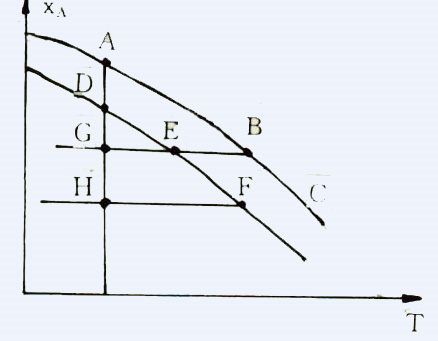
\includegraphics{figs/fig1.4.png}$$

4. 设多相催化反应\ce{A  <=> R}由下列步骤所构成：
\begin{itemize}
	\centering
	\item[(1)] $\ce{A + {$\sigma$} <=> A{$\sigma$}}$
		\item[(2)] $\ce{A{$\sigma$} <=> R{$\sigma$}}~~~~$
	\item[(3)] $\ce{R{$\sigma$} <=> R + {$\sigma$}}$
\end{itemize}

其中，表面反应步骤为速率控制步骤。试推导其动力学方程。


\newpage
\section{第三、四章}

\begin{question}
  一大一小两个釜式反应器串联，证明对于一级单一反应，反应器的串联顺序对生产结果没有影响。
\end{question}

\begin{question}
  在理想间歇反应器中进行液相均相反应
  \[
	  \ch{A + B -> P}
  \]
  反应速率方程为
  \[
	  r = k c_\mathrm{A} c_\mathrm{B} \quad \si{kmol.L^{-1}.s^{-1}}
  \]
  \[
	  k = \SI{5.2e14}e^{-13840/T}
  \]
  当反应物A和B的初始浓度$c_\mathrm{A0} = c_\mathrm{B0} = 4$\si{mol.L^{-1}}，而A的转化率$X_\mathrm{A} = 0.8$时，该间歇反应器平均每分钟可处理\SI{0.684}{kmol}的反应物A。
  
  (1) 若将该反应移到理想流动管式反应器中进行，仍维持348K等温操作，处理量和转化率同上，求所需反应体积。
  
  (2) 若该反应在绝热条件下进行，求A的转化率$X_\mathrm{A} = 0.8$时反应器的出口温度。进料温度348K，混合物密度$\rho = \SI{1800}{kg.m^{-3}}$，物料平均定压比热容为$\bar C_{p\mathrm{t}} = \SI{4.2}{kJ.kg^{-1}.K^{-1}}$，$\Delta H = \SI{-125.6}{kJ.mol^{-1}}$。
\end{question}

\begin{question}
  一活塞流反应器和一全混流反应器用两种方式串联。

  (a) 活塞流反应器在前，全混流反应器在后
  
  (b) 全混流反应器在前，活塞流反应器在后
  
  今分别在其中进行一级不可逆反应：
  \[
	  \ch{A -> B}
  \]
  己知$k = 2 \si{h^{-1}}$，$c_\mathrm{A0} = \SI{10}{mol/L}$，物料在每个反应器中的停留时间均为\SI{30}{min}，若两反应器温度相同，反应过程中物料密度基本不变，试计算两种情况下的出口浓度。
\end{question}

\begin{question}
	某液相均相反应\ch{A -> P}为一级不可逆反应，当反应温度100℃时，反应速率常数为\SI{0.4}{h^{-1}}，进料物料中A的初始浓度为2 mol/L。要求P的产量为480 mol/h，最终转化率为80\%。求下列几种情况下的反应体积：
  
	（1）反应在间歇釜式反应器中进行，辅助时间为1h；
  
	（2）反应在全混流釜式反应器中进行；
  
	（3）反应在活塞流管式反应器中进行。 

\end{question}


\begin{answer}
(1)
\[
    \begin{aligned}
      t&=\frac{1}{k}\frac{1}{\ln (1-x_{A})}=\frac{1}{0.4}\frac{1}{\ln (1-0.8)}=4\:\mathrm{h} \\
      Q_{0}&=\frac{F_{A0}}{C_{A0}} \\
      F_{A0}&={\frac{F_{P}}{X_\mathrm{Af}}}={\frac{480}{0.80}}=600\:\mathrm{mol/h} \\
      Q_{0}&={\frac{F_{A0}}{C_{A0}}}={\frac{600}{2}}=300\:\mathrm{L/h} \\
      V_{r}&=Q_{0}(t+t_{0})=300\times (4+1)=1500\:\mathrm{L}
    \end{aligned}
\]
\qquad (2)
\[
  \begin{aligned}
    \frac{V_{r}}{F_{A0}}&=\frac{X_\mathrm{Af}}{kC_{A0}\big(1-X_\mathrm{Af}\big)}=\frac{0.8}{0.4\times2\times(1-0.8)}=5 \\
    V_{r}&=5\times600=3000\:\mathrm{L}
    \end{aligned}
\]
\qquad (3)
\[
\begin{aligned}
  \tau&=\frac{1}{k}\frac{1}{\ln (1-X_\mathrm{A})}=\frac{1}{0.4}\frac{1}{\ln (1-0.8)}=4\:\mathrm{h}\\
  V_{r}&=Q_{0}\tau=300\times4=1200\:\mathrm{L}
\end{aligned}
\]
\end{answer}


\begin{question}
  液相反应
  \[
	  \ch{A + B -> R} \quad \text{(主反应)} \qquad r_\mathrm{R} = k_1c_\mathrm{A}^{0.6}c_\mathrm{B}^{1.2}
  \]
  \[
	  \ch{A + B -> S} \quad \text{(副反应)} \qquad r_\mathrm{S} = k_2c_\mathrm{A}^{2.0}c_\mathrm{B}^{0.2}
  \]
  
  (1) R为目标产物，选择合适的反应器型式和操作方式。
  
  (2) 如果反应活化能$E_1 < E_2$，应如何选择操作温度？
\end{question}



\end{document}
